\documentclass[11pt]{article}
\usepackage[margin=1in]{geometry}
\usepackage{graphicx}
\usepackage{subcaption}
\usepackage{dirtree}
\usepackage{url}
\usepackage{hyperref}

\usepackage{glossaries}

\makeglossaries{}

\newglossaryentry{CI/CD}{
  name={CI/CD},
  description={Continuous Integration and Continuous Development. The process of
  automating software testing, building, and deployment.}
}

\newglossaryentry{CLI}
{
    name={CLI},
    description={A command-line interface (CLI) is a text-based user interface (UI) used to run programs, manage computer files and interact with the computer.}
}

\newglossaryentry{DSL}
{
    name=DSL,
    description={A computer language that is specialized to a particular application/domain}
}

\newglossaryentry{target execution}
{
    name=target execution,
    description={An instance of a \gls{target} that needs to be completed as per described in the project definition}
}

\newglossaryentry{cache}
{
    name=cache,
    description={to save something to computers memory or local storage. An example would be the output of a \gls{target execution}}
}

\newglossaryentry{project definition}
{
    name=project definition,
    description={A file containing information pertaining a project, an example could be the language that was used}
}

\newglossaryentry{metadata}
{
    name=metadata,
    description={any custom data that the project owner wants to add about the project}
}

\newglossaryentry{target}
{
    name=target,
    description={An execution target, a recipe or command for what you want to do to/with the project, ie build and deploy the project, run tests, ect}
}

\newglossaryentry{monorepo}
{
  name=monorepo,
  description={A software-development strategy in which the code for a number of projects is stored in the same repository.}
}

\title{\textbf{4ZP6 Capstone Project}}
\author{Usman Asad --- asadu  --- 400199934\\
Ali Khan --- khana238  --- 400211680\\
Omar Alkersh --- alkersho --- 400214491 \\
Ahmed Al-sabounchi --- alsaboaa --- 001327403 \\
Tanveer Shakeel --- shakeelt --- 400226915}

\begin{document}

\maketitle
\tableofcontents
\newpage
\section{Introduction}
\subsection{Purpose}

There is no specific client for this software. The final product should be a
compiled binary tool to help manage monorepos.

\subsection{Document Convention}

No special convention.

\subsection{Intended Audience and Reading Suggestions}

This document is intended for the software developers who will be designing and
implementing the software to meet the requirements specified here. It is also
intended for assessors who will use this document to assess the fitness of this
project for the capstone and evaluate the final product.

\textbf{Reading suggestions:}
\begin{itemize}
  \item \href{https://en.wikipedia.org/wiki/Monorepo}{Monorepo WikiPedia}
  \item \href{https://www.redhat.com/en/topics/devops/what-is-ci-cd}{Redhat:
      What is CI/CD?}
\end{itemize}

\subsection{Product Scope}

A compiled CLI tool to manage and build projects of different languages in a
single monorepo. It should allow the user to define custom build \glspl{target}.
It should be able to execute \glspl{target} concurrently and allow the user to
define \gls{target} dependencies.

\subsection{References}

\textbf{Similar projects}:
\begin{itemize}
\item \href{https://nx.dev/}{NX}
\item \href{https://rushjs.io/}{rushJS}
\item \href{https://bazel.build/}{Bazel}
\end{itemize}

\section{Overall Description}

A compiled CLI tool to manage and build projects of different languages in a
single monorepo. It should allow the user to define custom build \glspl{target}.
It should be able to execute \glspl{target} concurrently and allow the user to
define \gls{target} dependencies.

There are other products that fulfill a similar goal, but none of them combines
the feature set of this product.

For \textbf{NX}, it is a node application that takes a long time to install in
CI/CD pipelines due to the large \texttt{node\_modules} required installation.

\textbf{RushJS} only manages JS projects. We want to manage any project in any language.

\textbf{Bazel} seems like the closest one, but it fails to alter the project
code. Which limits project initialization preparation, such as code generation
and transpilation for Typescript.

\subsection{Product Functions}

The final product should resemble NX the most, but with the advantage of being
faster and a smaller install. This should speed up CI/CD pipelines
significantly. Currently, installing NX and its dependencies could take up 10
minutes.

The functions are elaborated in the \hyperref[fig:feature]{Feature Model} subsection.

\subsection{User Classes and Characteristics}

The primary stakeholders or users for this project would be software engineers,
or software engineering companies that use a monorepo and wish to automate
development.

\subsection{Operating Environment}

The product should be called in a terminal, or via automation scripts, in a Unix
environment. It should work on x86\_64 compatible machines.

\subsection{Design Implementation Constraints}
See \hyperref[sec:constraints]{Constraints} section.

\subsection{User Documentation}

It should provide a CLI help flag detailing the available command and
functionality. It may include a manpage as well. A website with more
documentation can be provided in the future.

\subsection{Assumptions and Dependencies}

See \hyperref[sec:constraints]{Constraints} section.

\section{Requirements}
\subsection{UI}

It is CLI application. There is not form of GUI or TUI.

\subsection{Hardware Interfaces}

See \hyperref[sec:constraints]{Constraints} section.

\subsection{Functional Requirements}
\label{sec:fun_req}
\begin{enumerate}
    \item The program must be compiled
    \item The program must have a \Gls{CLI}
    \item The user should be able to add projects to the monorepo using the \Gls{CLI} tool
    \item Each project should be able to be made in any programming language
    \item The user must be able to define \glspl{target} (example targets; run tests, build project, deploy project, ect) on each individual project.
    \item The program must be able to define project dependencies (ie a project in the monorepo uses and depends on another project in the repo)
    \item The program must be able to detect dependency changes
    \item The program must be able to produce a correct project dependency graph
    \item The user must be able to define project dependencies
    \item The concurrent execution must respect dependencies
    \item The program must be able to list all registered projects in the monorepo
    \item The program must return the status of the \gls{target execution}
    \item The program must preserve coloured output from the \glspl{target execution} status
    \item The program must be able to read \glspl{project definition} from a file
    \item The program should be able to detect malformed \glspl{project definition} and inform the user
    \item The project definition should contain the following information about the project; name, owner(s), version, main programming
    language, \glspl{target}, dependencies, tags and custom \gls{metadata}
    \item The user must be able to define custom execution \glspl{target} for each project.
    \item The program must be able to execute the \glspl{target} defined in the project
    \item The user must be able to define a \gls{target} output artifact
    \item The program must be able to print the \gls{target} output in realtime
    \item The project must be able to execute \glspl{target} concurrently
    \item \Gls{target execution} should fail if any of its dependencies failed to execute successfully
    \item The program must be able to \gls{cache} \gls{target execution} output whenever possible
    \item The program should store a workspace file for the monorepo containing information about the following; owners, app version,
    projects, tags, Git Repo Owner/URL, and required targets
\end{enumerate}

\subsection{Non Functional Requirements}
\begin{enumerate}
    \item The \glspl{project definition} should be stored as a JSON, YAML, and a custom \Gls{DSL} file.
    \item The colors used in the CLI output should be intuitive and aesthetic
    \item The \glspl{target execution} should execute in a timely fashion
\end{enumerate}

\subsection{Constraints}
\label{sec:constraints}
\begin{enumerate}
    \item The OS must be Unix based
    \item System must be x86 or arm64 compatible
    \item Git has to be installed on system
    \item Program must be called from within a git repo
    \item The user must be able to use the CLI to use program
    \item The program must be use git to track changes
    \item The program must be executed within a git repository
\end{enumerate}

\subsection{Communication Interfaces}

There are no communication interfaces.

\section{System Features}

Features marked as \emph{optional} are planned, but left as tentative to avoid
over planning. These features are not essential for the product, but are nice to
haves. Sub-sub sections are features that depend on their parent feature. This
is shown in the \hyperref[fig:feature]{features model graph}.\\

\subsection{Run \Glspl{target} on Projects}

See \hyperref[sec:fun_req]{function requirements} 17-23 and
\hyperref[fig:act_exec]{Execute targets diagram}.

\subsubsection{Execution Summary \emph{Optional}}

Print an execution summary for the projects. It should include the number of
failed \glspl{target execution} and which \glspl{target} failed.

\subsection{List Affected Projects}

See \hyperref[sec:fun_req]{function requirements} 6, 7, and 9. And
\hyperref[sec:constraints]{constraint} 3 and 6. Git will be used to detect code changes.

See \hyperref[fig:act_aff]{affected project activity diagram} for more
information about this feature.

\subsection{List Projects \emph{Optional}}

See \hyperref[sec:fun_req]{function requirements} 11 and 8.

\subsubsection{Filter projects based on attribute \emph{Optional}}

The user should be able to filter the projects based on the attributes specified
in the project definition.

\subsection{Support File Format For Definitions}

At least on of YAML, JSON, or a \gls{DSL} to record the project and workspace definitions.

\subsection{Validate project files \emph{Optional}}

See \hyperref[sec:fun_req]{function requirements} 15.

\subsubsection{Suggest Fixes}

Suggest file fixes to the malformed files.

\subsection{Specify command output format, \emph{Optional}}

The user should be able to specify the output of the execution results. They
should be able to specify whether to output in a human or machine readable
format.

\subsection{Run target(s) on affected projects \emph{Optional}}

After detecting the affected projects, run the specified target on these
projects, respecting the dependency graph.

\section{Other Nonfunctional Requirements}

\subsection{Performance Requirements}

\begin{itemize}
\item The product must be able to produce the dependency graph in a timely manner.
\item The product must be able to be installed quickly
\item The product must not have a large installation size
\end{itemize}

\subsection{Safety Requirements}

There are no safety requirements.

\subsection{Security Requirements}

There are no security requirements.

\subsection{Software Quality Attributes}

There are no software quality attributes.

\newpage
\section{Diagrams}

\subsection{State Diagram}
Describes the possible states of the program

\begin{figure}[htbp]
  \centering
  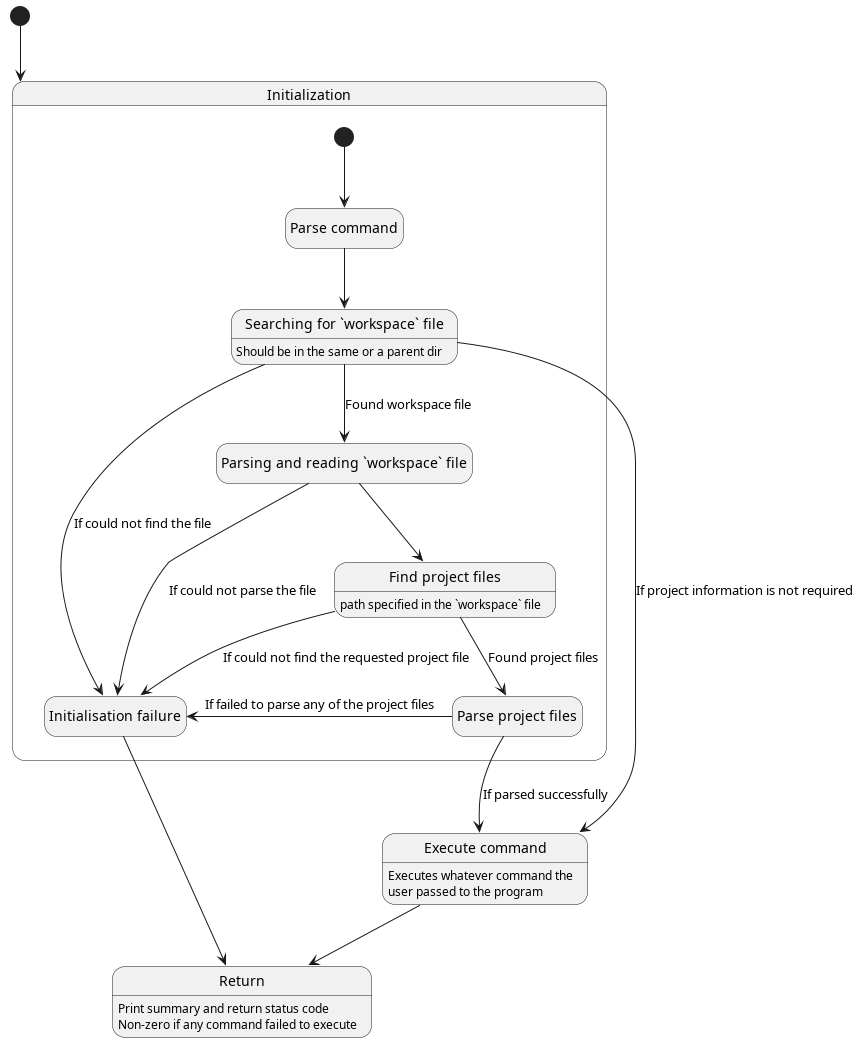
\includegraphics[width=0.5\textheight]{diags/state.png}
  \caption{\label{fig:state}State diagram}
\end{figure}

\newpage
\subsection{Activity Diagram}

Note that the activity diagram are broken into pieces for readability on PDF.
You can follow the figure order.

\subsubsection{Get Affected projects}

Describes how the program gets a list of affected projects.

\begin{figure}[htbp]
  \centering
  \begin{subfigure}{0.45\linewidth}
    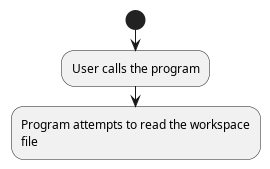
\includegraphics[width=\linewidth]{diags/get_affected_activity.png}
    \caption{Initialize}
  \end{subfigure}
  \begin{subfigure}{0.45\linewidth}
    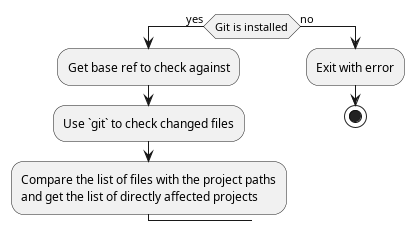
\includegraphics[width=\linewidth]{diags/get_affected_activity_001.png}
    \caption{Check Changes}
  \end{subfigure}
  \begin{subfigure}{0.5\linewidth}
    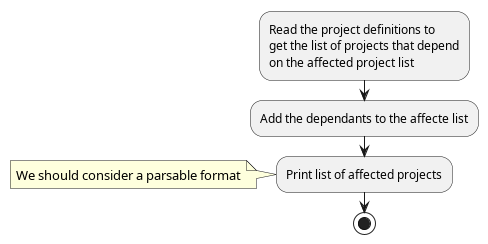
\includegraphics[width=\linewidth]{diags/get_affected_activity_002.png}
    \caption{Check Dependencies}
  \end{subfigure}
  \caption{\label{fig:act_aff}Get a List of Affected Projects}
\end{figure}

\subsubsection{Execute targets}

Shows the activity of the program when executing projects \glspl{target}.

\begin{figure}[htbp]

  \begin{minipage}{0.45\textwidth}
    \centering
    \begin{subfigure}[b]{\linewidth}
      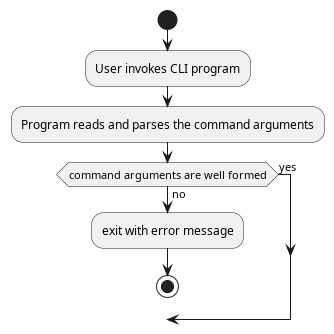
\includegraphics[width=\linewidth]{diags/activity.png}
      \caption{Get user input}
    \end{subfigure}

    \bigskip
    \addtocounter{subfigure}{1}

    \begin{subfigure}[b]{\linewidth}
      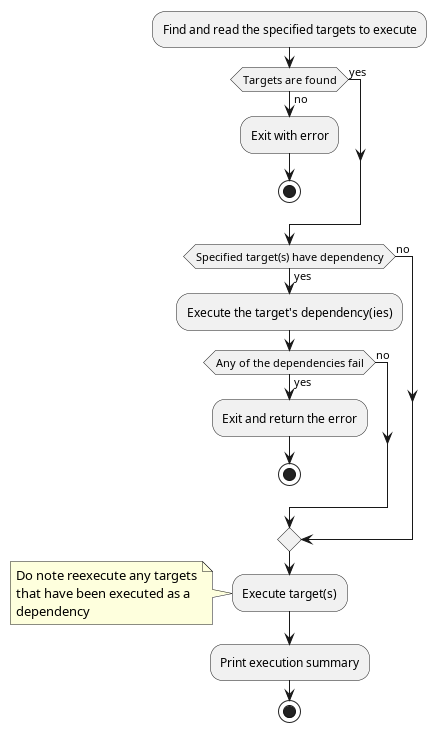
\includegraphics[width=\linewidth]{diags/activity_002.png}
      \caption{Execute}
    \end{subfigure}
  \end{minipage}
  \hfill
  \begin{minipage}{0.5\textwidth}
    \addtocounter{subfigure}{-2}
    \begin{subfigure}[b]{\linewidth}
      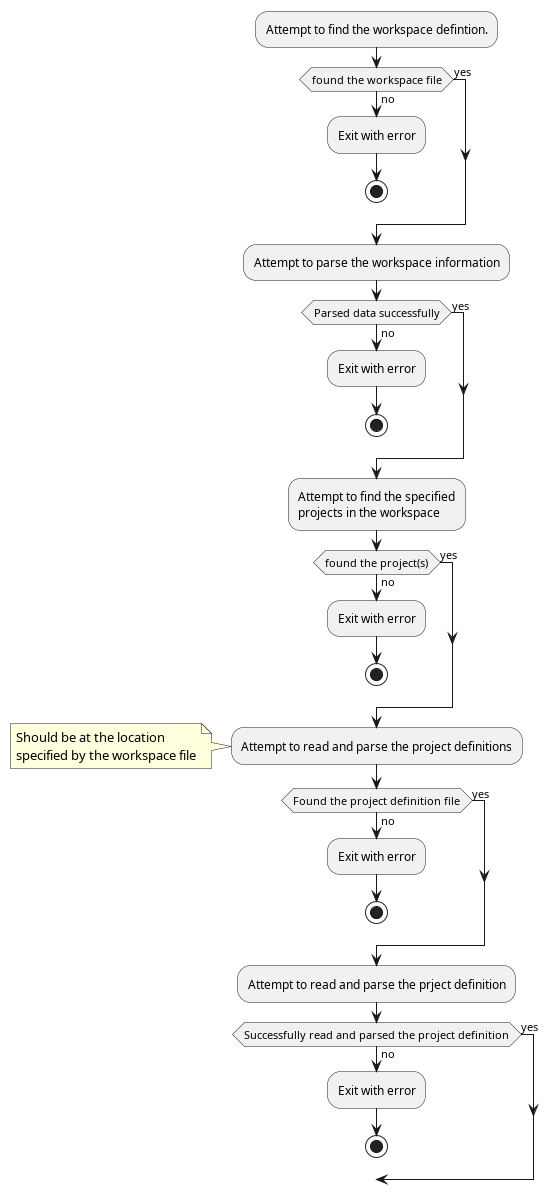
\includegraphics[width=\linewidth]{diags/activity_001.png}
      \caption{Initialize}
    \end{subfigure}
  \end{minipage}

  \caption{\label{fig:act_exec}Execute Project Targets}
\end{figure}

\clearpage

\subsection{Sample Repository Structure}

Sample project directory structure:

\dirtree{%
  .1 repo/.
  .2 .git/.
  .2 workspace\_def
  \ldots{}
  \begin{minipage}[t]{7cm}
    This file contains information about the entire
    repository{.}
  \end{minipage}.
  .2 path/to/.
  .3 proj1/.
  .4 src/...
  .4 proj\_def
  \ldots{}
  \begin{minipage}[t]{7cm}
    This file contains the project definition as described by
    the some previous section{.} All targets are executed from
    this location{.}
  \end{minipage}.
  .3 proj2/.
  .4 src\_file.
  .4 proj\_def.
}

\clearpage
\subsection{Feature Model}

This shows and elaborates on the intended features of this program. See
\url{https://en.wikipedia.org/wiki/Feature_model} for information about
``Feature Models''.

\begin{figure}[htbp]
  \centering
  \begin{subfigure}{\linewidth}
    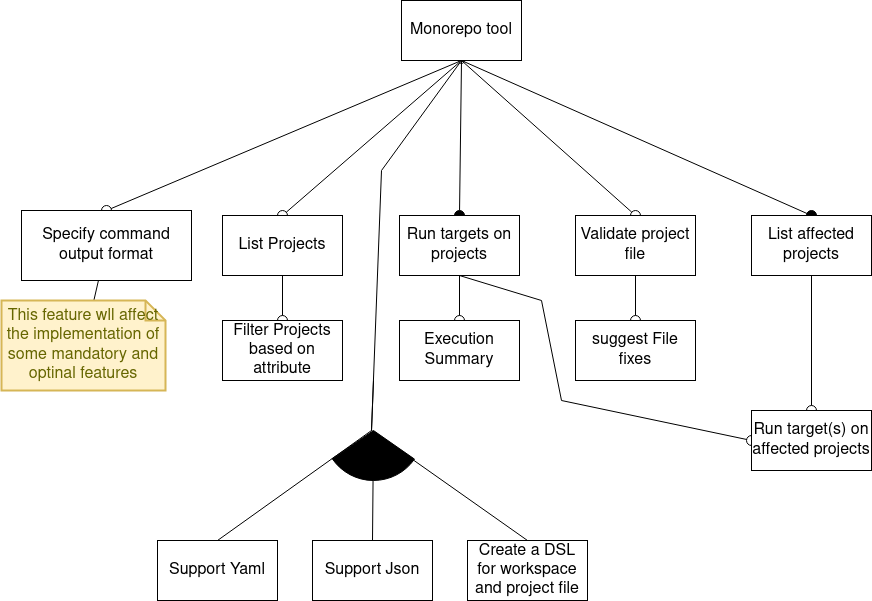
\includegraphics[width=\linewidth]{diags/feature.png}
    \caption{\label{fig:feature}Specifies the features of the program.}
  \end{subfigure}
  \\[5ex]
  \begin{subfigure}{\linewidth}
    \centering
    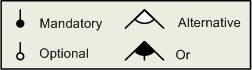
\includegraphics[width=0.3\linewidth]{diags/features_legend.jpg}
    \caption{Features Model Legend}
  \end{subfigure}
  \caption{Feature Model}
\end{figure}

\clearpage
\section{Glossary}
\printglossary[title=\normalsize\vspace*{-1.5\baselineskip}, toctitle=]

\end{document}
